\documentclass[12pt]{article}

\usepackage{fullpage}
\usepackage{multicol,multirow}
\usepackage{tabularx}
\usepackage{ulem}
\usepackage{listings}
\usepackage{pgfplots}
\usepackage[utf8]{inputenc}
\usepackage[russian]{babel}

% Оригиналный шаблон: http://k806.ru/dalabs/da-report-template-2012.tex

\begin{document}

\section*{Лабораторная работа №1, по курсу дискрeтного анализа: Сортировки за линейное время}

Выполнил студент группы М8О-212Б-22 МАИ \textit{Мамонтов Егор}.

\subsection*{Условие}

\textbf{Вариант:} 6-2 

Требуется разработать программу, осуществляющую ввод пар «ключ-значение», их упорядочивание по возрастанию ключа указанным алгоритмом сортировки за линейное время и вывод отсортированной последовательности.
Вариант задания определяется типом ключа (и соответствующим ему методом сортировки) и типом значения:
Поразрядная сортировка.

Тип ключа: телефонные номера, с кодами стран и городов в формате +<код страны> <код города> телефон.

Тип значения: строки переменной длины (до 2048 символов).

\newpage
\subsection*{Метод решения}

Для решения задачи нужно создать два вектора, в первом векторе я буду хранить ключи и значения в виде \texttt{std::pair}.
Второй вектор нужен для хранения ключа в виде \texttt{unsigned long long} и номер строки из основного вектора тоже через \texttt{std::pair}.
Далее я передаю в поразрядную сортировку второй вектор. После сортировки вывожу строки из первого массива по номерам из второго массива.
Тем самым я экономлю память, не таская длинные строки внутри сортировки.

\newpage
\subsection*{Описание программы}

Исходные данные хранятся в структуре \texttt{std::pair<std::string, std::string>}.
Дополнительный вектор для сортировки, состоящий из структур данных \texttt{std::pair<unsigned long long, int>}.
Программа состоит из следующих функций:
\begin{enumerate}
    \item \texttt{unsigned long long getMax(std::vector<std::pair<unsigned long long, int>>& array)}
    - функция возвращает максимальный элемент из вектора.
    \item \texttt{void input(std::vector<std::pair<std::string, std::string>>& array)}
    - функция совершает ввод ключей и значений из консоли в основной вектор.
    \item \texttt{unsigned long long to\_ull(std::string s)}
    - функция переводит std::string в unsigned long long.
    \item \texttt{void countSort(std::vector<std::pair<unsigned long long, int>>& array, unsigned long long exp)}
    - функция сортировки подсчётом по каждой цифре числа, начиная с конца.
    \item \texttt{void radix\_sort(std::vector<std::pair<unsigned long long, int>>\& arr)}
    - функция поразрядной сортировки для строки, сортирует значения строк в массиве передавая индексы в функцию сортировки подсчётом.
    \item \texttt{int main()}.
\end{enumerate}

\newpage
\subsection*{Дневник отладки}

\begin{itemize}
    \item Сначала я сталкивался с проблемой \texttt{RE} теста №3. Чтобы решить проблему, нужно было учесть пустые введённые строки (очень хотелось бы, чтобы об этом указывалось в задании.)
    \item Далее я сталкивался с проблемами \texttt{WA} теста №7. Решением было не выкорёживаться, и нормально хранить все строки, как они задавались изначально, без попыток превратить номер \texttt{79851234567} в \texttt{+7-985-1234567}. 
    \item Далее программа, путём эксперемента с вариантом моего товорища, получила вердикт "\texttt{OK}".
    \item Далее я пытался эксперементировать с программой, пытался её ускорить и ещё сильнее оптимизировать. По итогам этих манипуляций получилось ускорить программу со 1.5 секунды до 1.1 секунды, без ущерба по памяти.
    \item Я разработал ещё один способ, как ускорить программу, путём работы с дополнительным вектором не как с \texttt{std::vector<std::pair<unsigned long long, int>>} , а как c \texttt{std::vector<unsigned long long>}, записывая номер строки в конец \texttt{unsigned long long}. Но тогда программа ограничится максимумом в 999.999 элементов.
\end{itemize}

\newpage

\begin{figure}
    \centering
    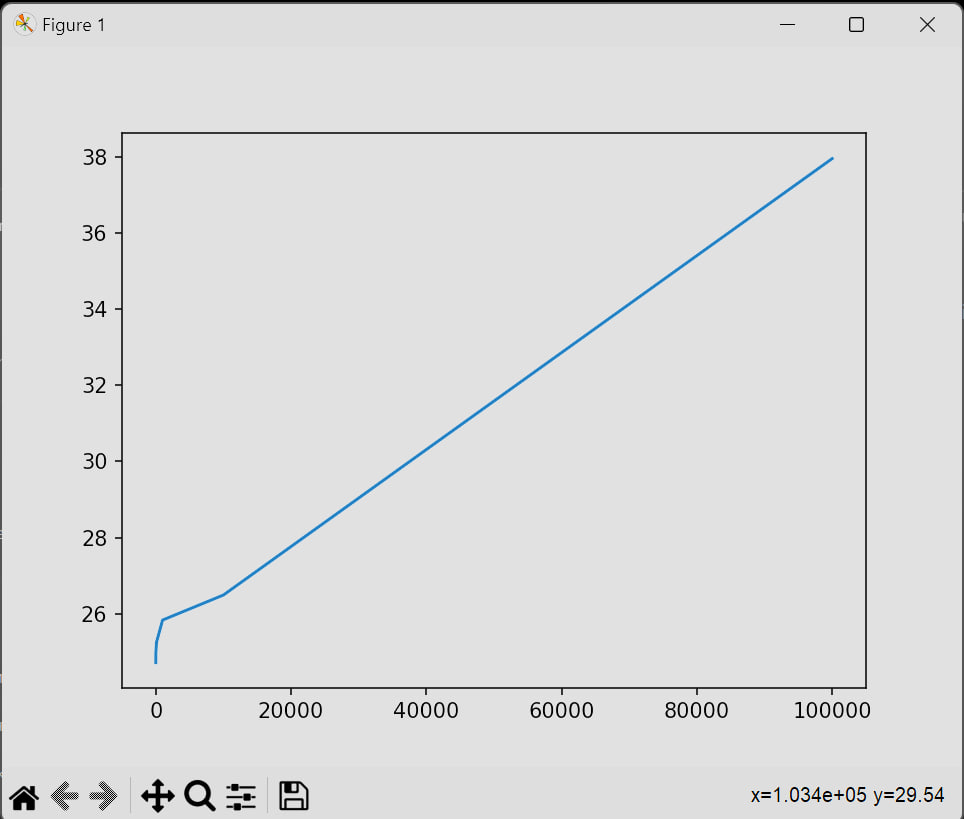
\includegraphics[width=\textwidth]{graph.png}
    \caption{Графики зависимости времени работы программы от количества введенных данных}
\end{figure}

\subsection*{Тест производительности}

Сложность написанного алогоритма $O(n)$. Для построения графика (Рис. 1) использовались тесты от 1 до 100000 строк с данными.
Из нескольких графиков видно, что количество входных данных почти не влияет на время работы программы.

\newpage
\subsection*{Выводы}

Поразрядная сортировка является ключевым методом для быстрой обработки массивов данных.
Этот метод гарантирует, что время сортировки будет расти пропорционально количеству обрабатываемых элементов, что идеально подходит для управления огромными и постоянно увеличивающимися данными.
Тем не менее, для более сложных структур данных, где требуется только сравнение элементов, более подходящими могут быть алгоритмы сортировки с временной сложностью $O(n \log n)$.

\end{document}
